\documentclass[11pt]{article}

% Use wide margins, but not quite so wide as fullpage.sty
\marginparwidth 0.5in 
\oddsidemargin 0.25in 
\evensidemargin 0.25in 
\marginparsep 0.25in
\topmargin 0.25in 
\textwidth 6in \textheight 8 in
% That's about enough definitions

% multirow allows you to combine rows in columns
\usepackage{multirow}
% tabularx allows manual tweaking of column width
\usepackage{tabularx}
% longtable does better format for tables that span pages
\usepackage{longtable}
\usepackage{graphicx}

\begin{document}

% this is an alternate method of creating a title
\hfill\vbox{\hbox{Huang, Jonathan}
      \hbox{CS5785: Modern Analytics}  
      \hbox{\today}}\par

\bigskip
\centerline{\Large\bf CS5785: Homework 0}\par
\bigskip

\section{Setting Up Python}

I signed up for Kaggle, installed Python (Canopy), and got it working with my preferred IDE (Sublime Text). On an interesting note, it turns out that getting Sublime to play nice with Canopy is a little annoying. 

\section{Iris Flowers}
\begin{enumerate}
\item[1] In this dataset, there are 4 features/attributes per sample (in addition to the specific class for each entry), 3 different iris classes, and 50 samples of each class recorded.

\item[2] The code for this problem can be found in HW0.py (which should be attached to this submission). Specifically, the parsing code is found on lines 5 (for the N x p array containing attributes) and 6 (for the N vector containing species).

\item[3] The plot for this problem is on the following page. The code used to generate this plot can be found in HW0.py. Specifically the code used was lines 14 to 38.

\newpage

\begin{figure}[h]
\centering
  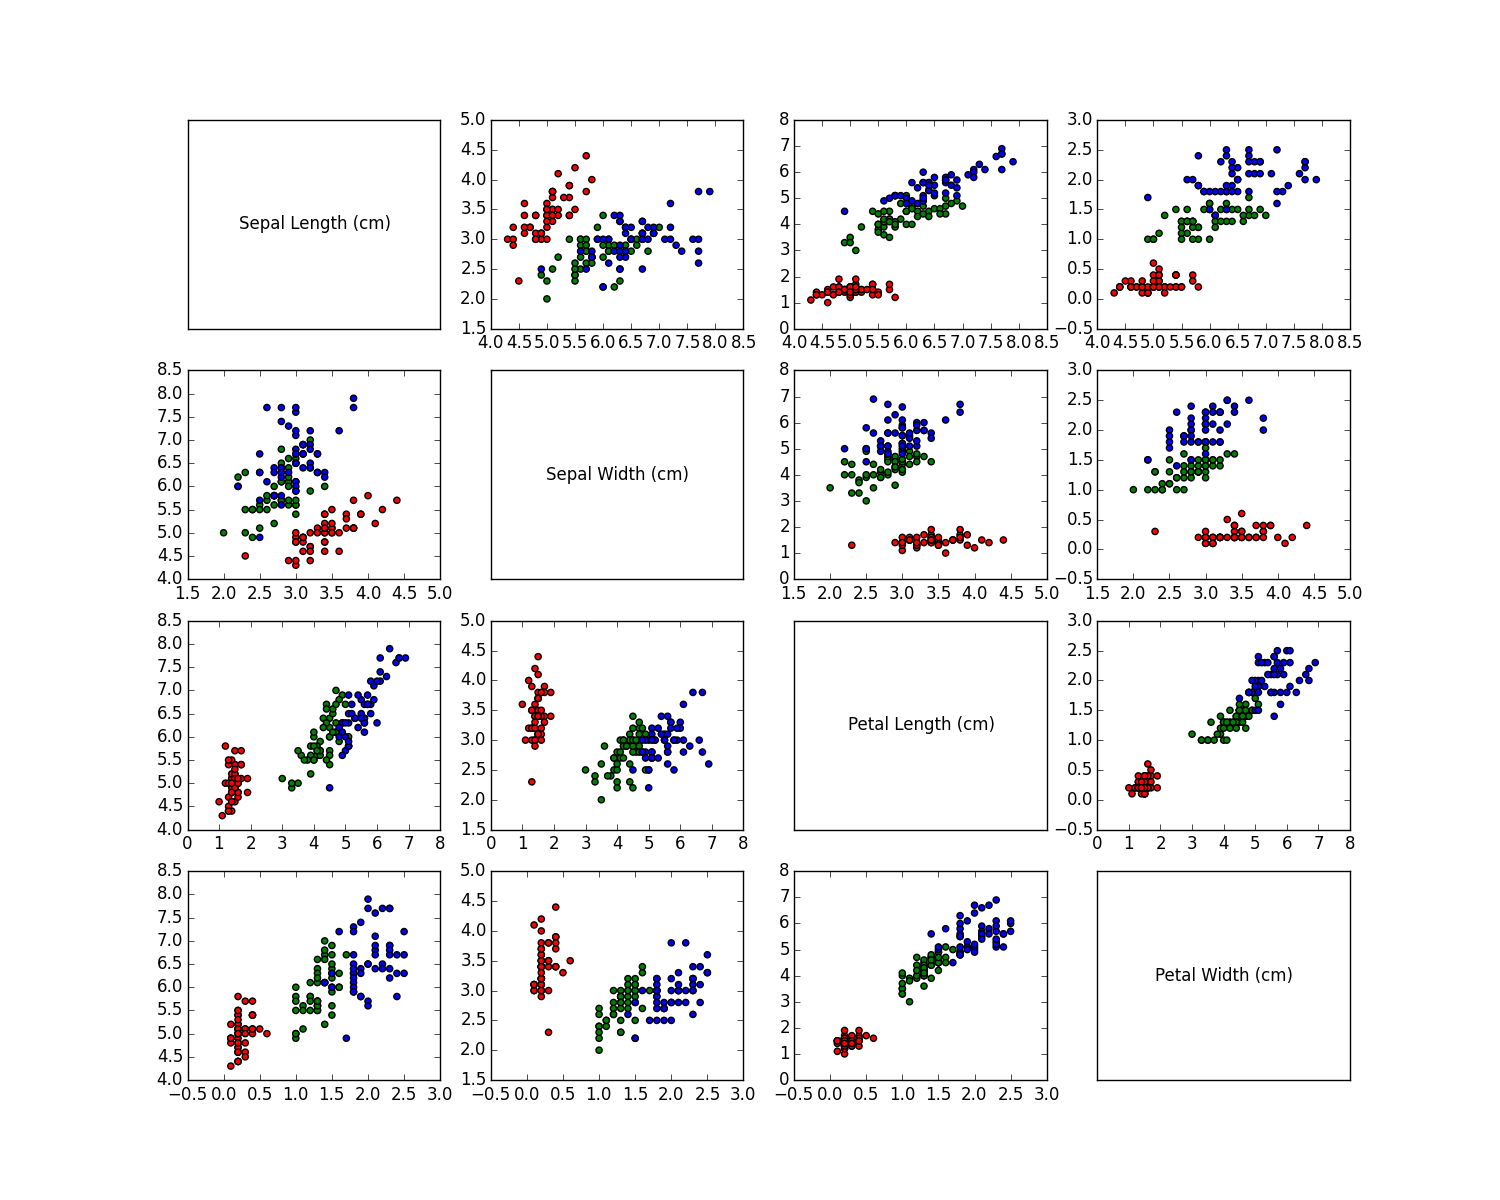
\includegraphics[scale=0.4]{HW0plot.png}
\caption{Plot 2.3: Iris Data (red = setosa, green = versicolor, blue = virginica)}
\end{figure}

\end{enumerate}

\end{document}
